\documentclass[11pt,letterpaper]{article}
\usepackage[utf8]{inputenc}
\usepackage[spanish]{babel}
\decimalpoint
\usepackage{amsmath}
\usepackage{amsfonts}
\usepackage{amssymb}
\usepackage{physics}
\usepackage{hyperref}
\usepackage[left=2cm,right=2cm,top=2cm,bottom=2cm]{geometry}

\usepackage{graphicx}
\graphicspath{{img_tarea03/}}


\usepackage[draft,inline,nomargin]{fixme} \fxsetup{theme=color}
\definecolor{jacolor}{RGB}{200,40,0} \FXRegisterAuthor{ja}{aja}{\color{jacolor}JA}

\newcommand{\mcM}{\mathcal{M}}

\renewcommand{\labelenumii}{\arabic{enumi}.\arabic{enumii}}
\renewcommand{\labelenumiii}{\arabic{enumi}.\arabic{enumii}.\arabic{enumiii}}
\renewcommand{\labelenumiv}{\arabic{enumi}.\arabic{enumii}.\arabic{enumiii}.\arabic{enumiv}}

%%%%% Author
\author{José Alfredo de León}

%%%% Title 
\title{Tarea 3\\
\large{Métodos de Simulación Computacional para Sistemas Cuánticos - 2022-2}}


\begin{document}
\date{08 de marzo de 2022}
\maketitle
 	
\section{Objetivos}
\subsection{Objetivo general}
Analizar en diferentes escenarios el ajuste de mínimos cuadrados.

\subsection{Objetivos específicos}
\begin{enumerate}
\item Estudiar el método de ajustes de mínimos cuadrados en el caso 
general.
\item Estudiar la factorización $LU$ de una matriz cuadrada.
\item Implementar sustitución para adelante y para atrás de
un sistema de ecuaciones con matrices triangulares 
inferior y superior, respectivamente.
\item Implementar la descomposición LU para la resolución de sistemas
de ecuaciones lineales.
\item Implementar el cálculo de la inversa de una matriz reciclando el código
de las subrutinas para eliminación de Gauss-Jordan.
\end{enumerate}

\section{Marco teórico}
\subsection{Descomposición LU}
Toda matriz cuadrada $M$ puede factorizarse como
\begin{align}
M=LU,
\end{align}
con $L$ y $U$ matrices triangulares inferior y superior, respectivamente.
Esta descomposición puede aprovecharse para resolver sistemas de ecuaciones
lineales de la forma $M\vec x=\vec b$; reescribimos esta ecuación
utilizando la factorización $LU$ de $M$ y tenemos
\begin{align}
L\qty(U\vec{x})&=\vec{b},
\end{align}
podemos resolver el sistema $M \vec x=\vec b$ resolviendo primero para $\vec y$
en la ecuación $L\vec y=\vec b$, con sustitución para adelante,
e inmediatamente después para $\vec x$ en la ecuación $U\vec x=\vec y$, 
utilizando sustitución para atrás. Este procedimiento resulta ser
computacionalmente menos costoso que el procedimiento de eliminación
de Gauss-Jordan. 

\subsection{Mínimos cuadrados}
El problema del ajuste de mínimos cuadrados consiste en
ajustar una función $f(x)$, tal que minimice a la función $\chi^2$ y que sea combinación 
lineal de algunas funciones base $X_k(x)$, a un conjunto de datos $\qty{(x_i,y_i)}$.
Si se toma una base de $M$ funciones $X_k(x)$, la función a ajustar es 
\begin{align}
y(x)=\sum_{k=0}^{M-1}a_kX_k(x).
\end{align}
El problema se reduce entonces a encontrar los parámetros $a_k$. Para 
esto utilizamos el método de mínimos cuadrados, que consiste en hallar los
valores de $a_k$ que minimizan el valor de la función $\chi^2$.
La función $\chi^2$ se define como
\begin{align}\label{eq:chi_squared}
\chi^2=\sum_0^{N-1}\qty[\frac{y_i-\sum_{k=0}^{M-1}a_kX_k(x)}{\sigma_i}],
\end{align}
donde $\sigma_i$ son los errores de las mediciones, usualmente la desviación
estándar. Si las $\sigma_i$ no se conocen pueden todas suponerse iguales a 1.
Siguiendo el procedimiento de optimización para la función $\chi^2$ en 
\eqref{eq:chi_squared} encontramos que el mínimo de esta función ocurre cuando
\begin{align}\label{eq:linear:sys:least:squares}
\sum_{j=0}^{M-1}a_{kj}a_j=\beta_k,
\end{align}
es una matriz de dimensión $M\times M$ y 
\begin{align}
\beta_k=\sum_{i=0}^{N-1}\frac{X_j(x_i)X_k(x_i)}{\sigma_i^2}
\end{align} 
un vector de tamaño $M$. Convenientemente podemos definir a la matriz $A$ como
\begin{align}\label{eq:A:def}
A_{i,j}=\frac{X_j(x_i)}{\sigma_i}
\end{align}
y al vector $\vec b$
\begin{align}\label{eq:b:def}
b_i=\frac{y_i}{\sigma_i}
\end{align}
para así escribir a la matriz $\alpha$ y al vector $\beta$ como
\begin{align}\label{eq:alpha:and:beta}
\alpha=A^T\cdot A && \beta=A^T\cdot b.
\end{align}
Una de las razones para adoptar la matriz $\alpha$ en nuestra discusión es que su matriz
inversa $C=\alpha^{-1}$, llamada matriz de covarianza, está relacionada
con las incertezas de los parámetros estimados $a_j$ del ajuste de mínimos 
cuadrados.  

En resumen, se necesitan dos ingredientes para hacer el ajuste de mínimos
cuadrados:
\begin{enumerate}
\item Un conjunto de $N$ datos $\mathcal{P}=\qty{(x_i,y_i)}$.
\item Una base de $M$ funciones a ajustar a los datos de $\mathcal{P}$.
\end{enumerate}
Seguidamente, se resuelve el sistema de ecuaciones lineales \eqref{eq:linear:sys:least:squares},
considerando las definiciones en \eqref{eq:A:def}, \eqref{eq:b:def} y
\eqref{eq:alpha:and:beta} para construir la ecuación matricial. Finalmente,
$\alpha^{-1}$ nos da idea de las incertezas en la estimación que se 
obtiene de los parámetros $a_j$ del ajuste.

\section{El problema}
Para este trabajo se quiere generar 50, 100 y 150 puntos de $x$ en el
intervalo $[-5,5]$ con la función 
\begin{align}
f(x,R)=0.4x^4-0.5x^3-x^2+1+R,
\end{align}
donde vamos a considerar que $R$ es un parámetro con amplitudes (i) $\pm 0.1$,
(ii) $\pm 1$ y (iii) $\pm 10$. El objetivo es hacer el ajuste de mínimos 
cuadrados a los 9 \textit{sets} de puntos considerando dos conjuntos 
diferentes de funciones base:
\begin{enumerate}
\item $1,x,x^2,x^3,x^4$
\item $L_0(x),L_1(x),L_2(x),L_3(x),L_4(x)$,
\end{enumerate}
con $L_i(x)$ los polinomios de Legendre.

\section{Implementación}
El problema principal a resolver es el ajuste de mínimos cuadrados, que
es calcular los parámetros $a_j$ resolviendo el sistema de ecuaciones
lineales \eqref{eq:linear:sys:least:squares}. Para resolver este sistema
utilizamos la descomposición $LU$ de la matriz $\alpha$. Por esta razón,
se implementaron las rutinas y subrutinas que encuentren la factorización 
$LU$ de una matriz y que resuelvan un sistema lineal de ecuaciones por medio
de sustitución para adelante y para atrás. Además, se implementaron
algunas rutinas para resolver las instrucciones específicas de la tarea.

Las rutinas implementadas para esta tarea fueron:
\begin{enumerate}
\item \verb|ForwardSubstitution|: realiza la sustitución para adelante
para encontrar la solución $\vec y$ de un sistema $L\vec y=\vec b$ con
$L$ una matriz triangular inferior.
\item \verb|BackwardSubstitution|: realiza la sustitución para atrás
para encontrar la solución $\vec x$ de un sistema $U\vec x=\vec y$ con
$U$ una matriz triangular superior.
\item \verb|MatrixToZeroUnderPivot2|: calcula la matriz que corresponde
a las operaciones entre filas para convertir en uno el elemento $(R,R)$ de
la matriz $M$ y convertir en cero todos los elementos por debajo de él.
Esta es una subrutina implementada en la tarea 1 que se modificó para 
los usos de la rutina \verb|LUdecomposition| de esta tarea.
\item \verb|LUdecomposition|: calcula la factorización $LU$ de una matriz $M$
siguiendo el procedimiento de eliminación Gaussiana tanto para encontrar 
la matriz $U$, como para iterativamente construir las matrices inversas
de las matrices correspondientes a las operaciones entre filas durante
la eliminación Gaussiana, el producto de estas matrices inversas
es igual a la matriz $L$. Debemos enfatizar que las matrices inversas
se calculan sin utilizar la rutina \verb|Inverse| de Mathematica.
\item \verb|LinearSolver[A]|: resuelve la ecuación $Ax=b$ utilizando
la factorización $LU$ de la matriz $A$.
\item \verb|GaussianElimination3[M,2, chapuz:-2]| realiza el procedimiento
de eliminación gaussiana para encontrar la inversa de una matriz.
\item \verb|BackElimination3[Udummy_, 2, inverse_]| realiza el procedimiento
de eliminación para terminar de encontrar la inversa de una matriz.
\item \verb|MyInverse[M]|: calcula la inversa de una matriz utilizando
el procedimiento de GaussJordan.
\item \verb|CovarianceMatrix[A]|: calcula la matriz de covarianza $\alpha$
dada la matriz $A$ como entrada.
\end{enumerate}
Otras subrutinas también fueron implementadas para evitar copiar código
una y otra vez a lo largo del Notebook. No se mencionan aquí porque no 
implementan ningún procedimiento que pueda ser útil fuera del alcance de esta
tarea. Refiérase al notebook para revisarlas.

\section{Resultados}
Los resultados al problema del ajuste de mínimos cuadrados de los 9 sets
de datos para las dos funciones mencionadas en la sección 3 se muestran
de en las Figs. 1 a la 18. 

En las Figs. 1 a la 9 se muestran los resultados
para el ajuste de mínimos cuadrados utilizando el polinomio $f(x)=a_0
+a_1x^1+a_2x^2+a_3x^3+a_4x^4$. En las primeras 3 Figs. se muestra
el ajuste hecho con 50 puntos en el data set. Debemos notar que, aunque
cualitativamente la curva parece ajustarse a los puntos, el error porcentual
es significativo en la
estimación de algunos de los parámetros cuando la amplitud de $R$ es 
mayor o igual a uno. Los errores porcentuales en la estimación de los
parámetros se mantiene por debajo de 0.15 para las Figs. 1, 4 y 7. Como
debió de esperarse, la mejor estimación se obtiene para la mayor cantidad
de datos y la menor amplitud para $R$ [vea la Fig. 7].


En las Figs. 10 a la 18 se muestran los resultados para el ajuste de mínimos
cuadrados utilizando la base de funciones de los primeros 5 polinomios 
de Legendre. En general, el comportamiento del ajuste de mínimos cuadrados se
comporta de manera similar que para las funciones polinomiales, sin embargo,
debemos resaltar que las Figs. 12, 15 y 18 evidencian que el error porcentual
en la estimación de los parámetros es mayor que la que de los ajustes 
en las Figs. 3, 6 y 9, de las funciones polinomiales. 

En resumen, observamos que, en general, el ajuste de mínimos cuadrados
presenta una mejor estimación cuando el número de datos aumenta y cuando
la desviación $\delta y_i$ es menor. Sin embargo, cuando la desviación 
$\delta y_i$ aumenta, el uso de las funciones polinomiales como funciones 
base muestra funcionar mejor que el de las funciones de Legendre. 
Deberá explorarse esto para otro tipo de funciones para determinar si 
es un ventaja general por encima de cualquier otra base de funciones.

Ahora, vamos a discutir sobre la matriz de covarianza y la relación 
con el error de los parámetros $a_j$ calculados. La matriz 
de covarianza para el primer set de datos, utilizado para ajustar
la función polinomial, es
\begin{align}
\left(
\begin{array}{ccccc}
 0.072 & 0. & -0.013 & 0. & 0. \\
 0. & 0.014 & 0. & -0.001 & 0. \\
 -0.013 & 0. & 0.004 & 0. & 0. \\
 0. & -0.001 & 0. & 0. & 0. \\
 0. & 0. & 0. & 0. & 0. \\
\end{array}
\right).
\end{align}
Nos vamos a limitar a los elementos de la diagonal, que son la 
varianza de los parámetros $a_j$. Considerando que estos son proporcionales
al error de $a_j$, los mejores valores estimados son entonces los de 
la Fig. 7.
Por otro lado, la matriz de covarianza para el segundo set de datos, 
utilizado para ajustar los polinomios de Legendre, es
\begin{align}
\left(
\begin{array}{ccccc}
 0.064 & 0. & -0.007 & 0. & 0. \\
 0. & 0.013 & 0. & 0. & 0. \\
 -0.007 & 0. & 0.002 & 0. & 0. \\
 0. & 0. & 0. & 0. & 0. \\
 0. & 0. & 0. & 0. & 0. \\
\end{array}
\right).
\end{align}
Similarmente, considerando los elementos de la diagonal como proporcionales
a los errores de los parámetros $a_j$ notamos que la mejor estimación
se consiguió en la Fig. 16.

\begin{figure}
\centering
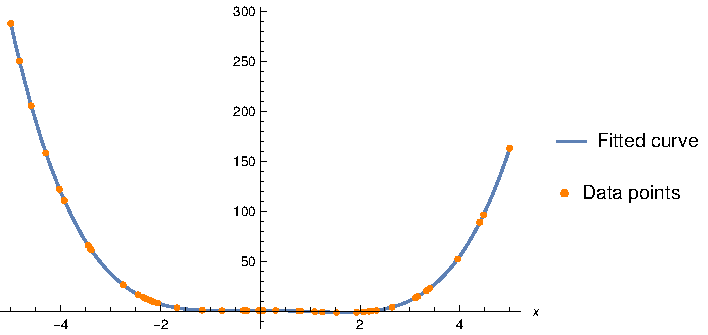
\includegraphics[width=11cm]{poly_01}
\caption{Base de funciones polinomiales grado 4, 50 puntos, $\delta R=\pm 0.1$,
curva ajustada: $f(x)=0.986273 - 0.00157755 x - 0.999636 x^2 - 0.499809 x^3 + 0.400026 x^4$.}
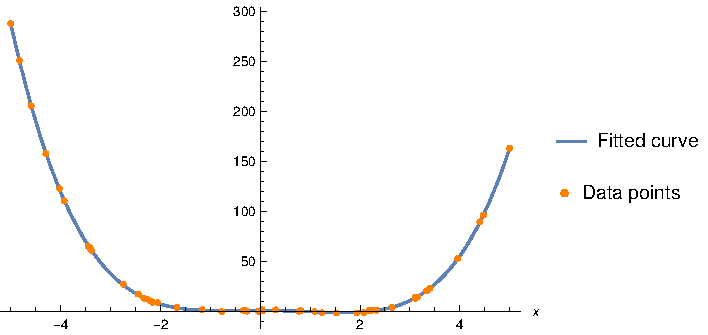
\includegraphics[width=11cm]{poly_02}
\caption{Base de funciones polinomiales grado 4, 50 puntos, $\delta R=\pm 1$,
curva ajustada: $f(x)=0.862413 - 0.0145073 x - 0.996247 x^2 - 0.498169 x^3 + 0.400259 x^4$.}
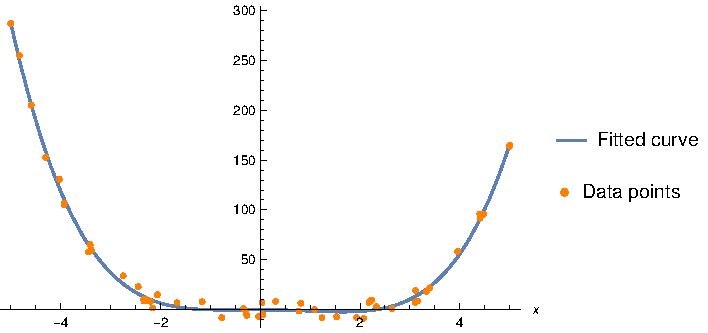
\includegraphics[width=11cm]{poly_03}
\caption{Base de funciones polinomiales grado 4, 50 puntos, $\delta R=\pm 10$,
curva ajustada: $f(x)=-0.376192 - 0.143804 x - 0.962351 x^2 - 0.481768 x^3 + 0.402582 x^4$.}
\label{fig:poly_50pts}
\end{figure}

\begin{figure}
\centering
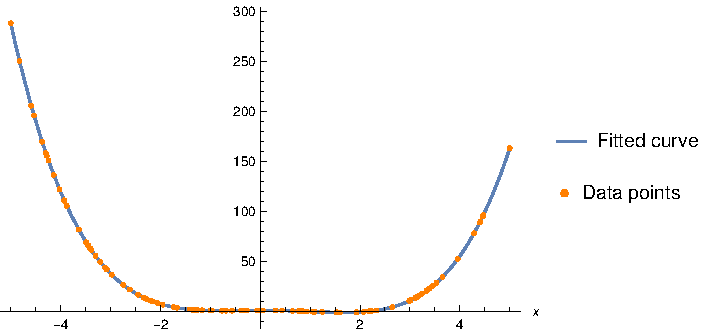
\includegraphics[width=11cm]{poly_04}
\caption{Base de funciones polinomiales grado 4, 100 puntos, $\delta R=\pm 0.1$,
curva ajustada: $f(x)=0.986895 - 0.00689854 x - 0.996389 x^2 - 0.499705 x^3 + 0.399873 x^4$.}
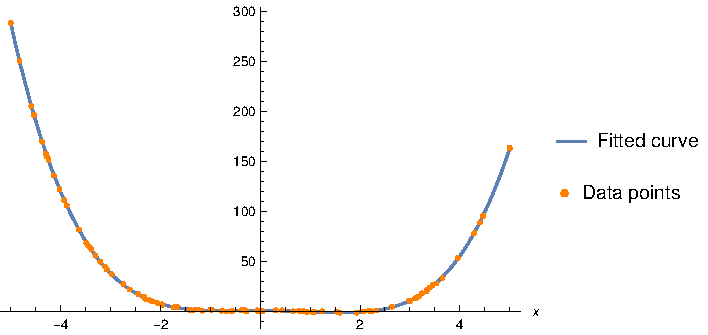
\includegraphics[width=11cm]{poly_05}
\caption{Base de funciones polinomiales grado 4, 100 puntos, $\delta R=\pm 1$,
curva ajustada: $f(x)=0.866069 - 0.0685425 x - 0.962956 x^2 - 0.497081 x^3 + 0.398685 x^4$.}
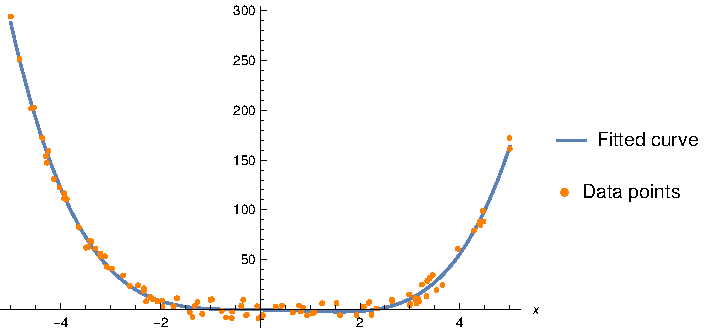
\includegraphics[width=11cm]{poly_06}
\caption{Base de funciones polinomiales grado 4, 100 puntos, $\delta R=\pm 10$,
curva ajustada: $f(x)=-0.342195 - 0.684982 x - 0.628628 x^2 - 0.470836 x^3 + 0.386812 x^4$.}
\label{fig:poly_100pts}
\end{figure}

\begin{figure}
\centering
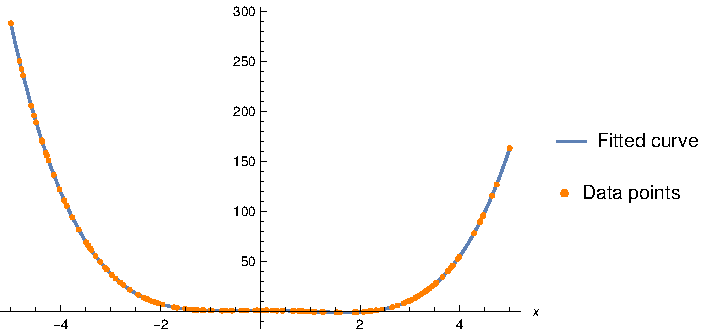
\includegraphics[width=11cm]{poly_07}
\caption{Base de funciones polinomiales grado 4, 150 puntos, $\delta R=\pm 0.1$,
curva ajustada: $f(x)=0.993142 - 0.00596376 x - 0.998524 x^2 - 0.499513 x^3 + 0.399911 x^4$.}
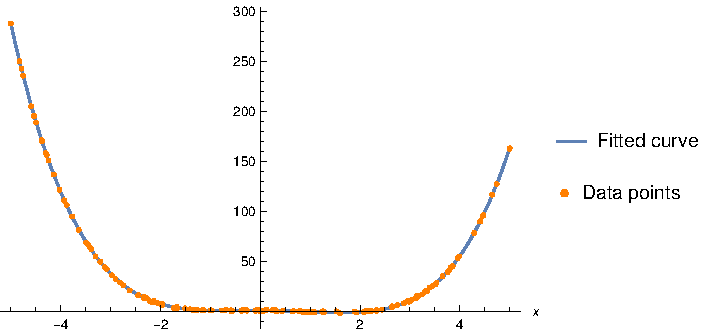
\includegraphics[width=11cm]{poly_08}
\caption{Base de funciones polinomiales grado 4, 150 puntos, $\delta R=\pm 1$,
curva ajustada: $f(x)=0.939325 - 0.0589197 x - 0.987856 x^2 - 0.495165 x^3 + 0.399229 x^4$.}
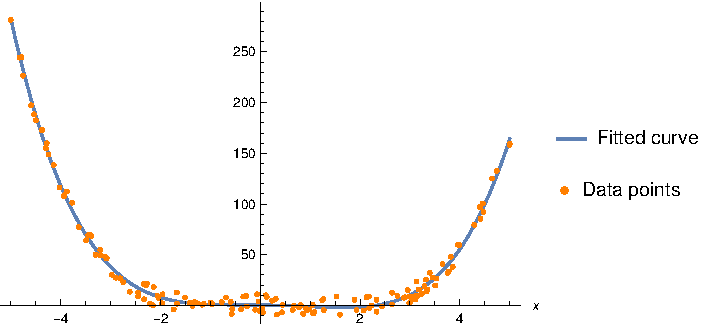
\includegraphics[width=11cm]{poly_09}
\caption{Base de funciones polinomiales grado 4, 150 puntos, $\delta R=\pm 10$,
curva ajustada: $f(x)=0.401153 - 0.588479 x - 0.881183 x^2 - 0.451691 x^3 + 0.3924 x^4$.}
\label{fig:poly_50pts}
\end{figure}

\begin{figure}
\centering
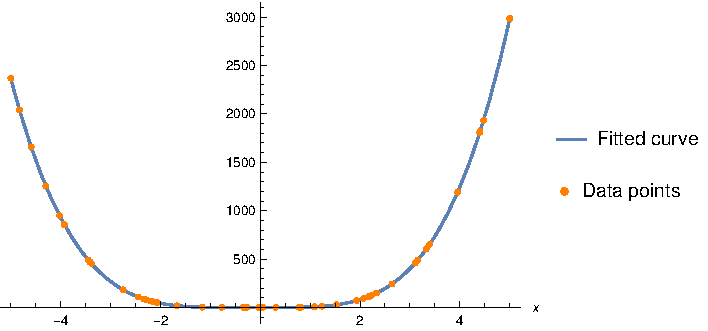
\includegraphics[width=11cm]{legendre_01}
\caption{Base de funciones polinomiales grado 4, 50 puntos, $\delta R=\pm 0.1$,
curva ajustada: $f(x)=0.98261 + 1.00066 x + 0.500542 (-1 + 3 x^2) + 
 0.500015 (-3 x + 5 x^3) + 0.124999 (3 - 30 x^2 + 35 x^4)$.}
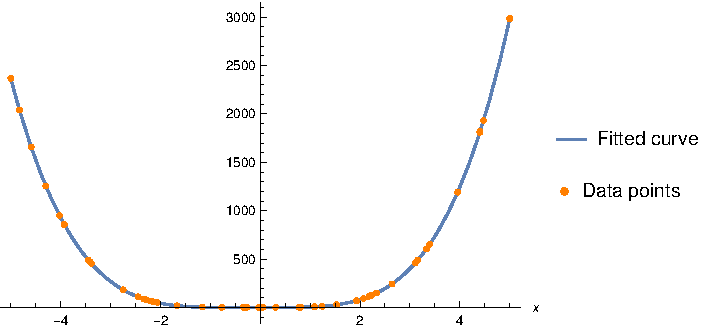
\includegraphics[width=11cm]{legendre_02}
\caption{Base de funciones polinomiales grado 4, 50 puntos, $\delta R=\pm 1$,
curva ajustada: $f(x)=0.859917 + 0.988717 x + 0.501739 (-1 + 3 x^2) + 
 0.500343 (-3 x + 5 x^3) + 0.125006 (3 - 30 x^2 + 35 x^4)$.}
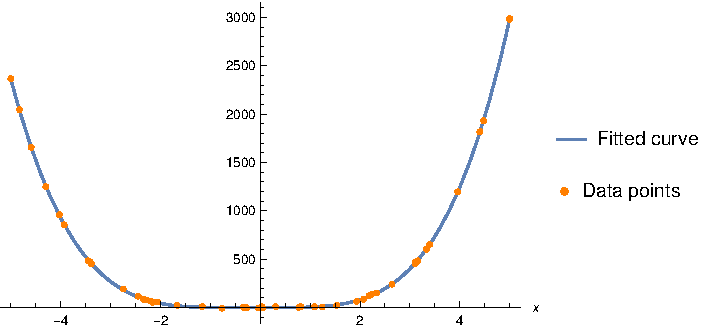
\includegraphics[width=11cm]{legendre_03}
\caption{Base de funciones polinomiales grado 4, 50 puntos, $\delta R=\pm 10$,
curva ajustada: $f(x)=-0.367014 + 0.869283 x + 0.513712 (-1 + 3 x^2) + 
 0.503623 (-3 x + 5 x^3) + 0.125072 (3 - 30 x^2 + 35 x^4)$.}
\label{fig:poly_50pts}
\end{figure}

\begin{figure}
\centering
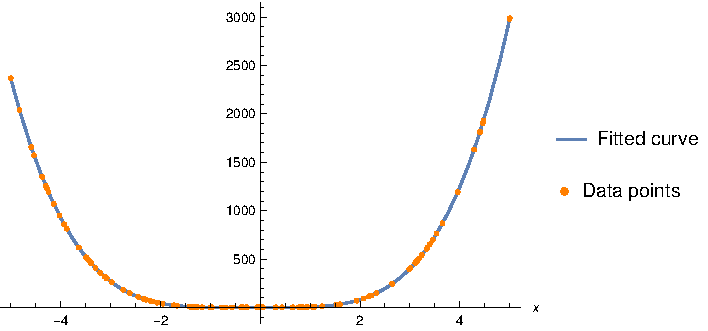
\includegraphics[width=11cm]{legendre_04}
\caption{Base de funciones polinomiales grado 4, 50 puntos, $\delta R=\pm 0.1$,
curva ajustada: $f(x)=0.987105 + 0.991816 x + 0.501268 (-1 + 3 x^2) + 
 0.500077 (-3 x + 5 x^3) + 0.124996 (3 - 30 x^2 + 35 x^4)$.}
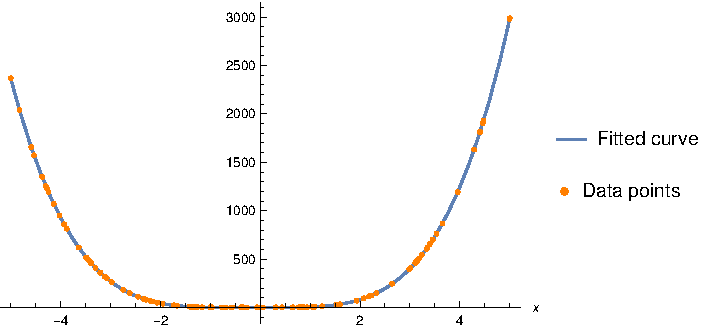
\includegraphics[width=11cm]{legendre_05}
\caption{Base de funciones polinomiales grado 4, 50 puntos, $\delta R=\pm 1$,
curva ajustada: $f(x)=0.877185 + 0.931741 x + 0.512073 (-1 + 3 x^2) + 
 0.500602 (-3 x + 5 x^3) + 0.124962 (3 - 30 x^2 + 35 x^4)$.}
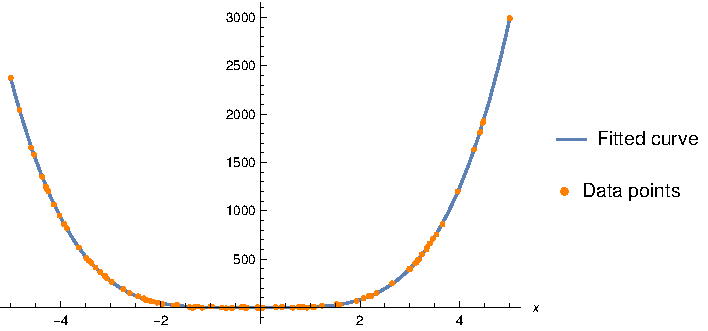
\includegraphics[width=11cm]{legendre_06}
\caption{Base de funciones polinomiales grado 4, 50 puntos, $\delta R=\pm 10$,
curva ajustada: $f(x)=-0.222015 + 0.330991 x + 0.620124 (-1 + 3 x^2) + 
 0.505851 (-3 x + 5 x^3) + 0.124623 (3 - 30 x^2 + 35 x^4)$.}
\label{fig:poly_50pts}
\end{figure}

\begin{figure}
\centering
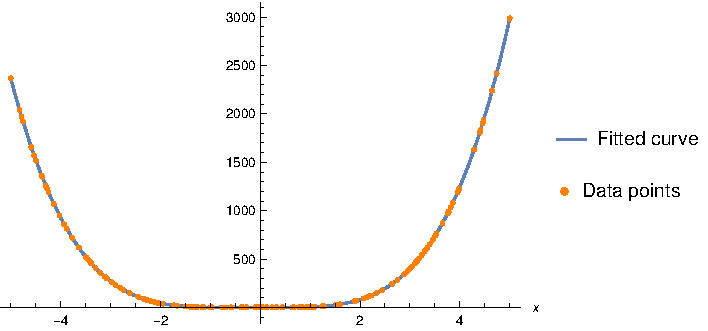
\includegraphics[width=11cm]{legendre_07}
\caption{Base de funciones polinomiales grado 4, 50 puntos, $\delta R=\pm 0.1$,
curva ajustada: $f(x)=0.995401 + 0.992907 x + 0.500262 (-1 + 3 x^2) + 
 0.500115 (-3 x + 5 x^3) + 0.124998 (3 - 30 x^2 + 35 x^4)$.}
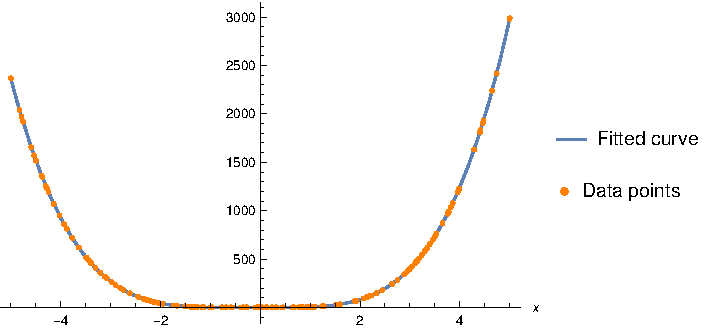
\includegraphics[width=11cm]{legendre_08}
\caption{Base de funciones polinomiales grado 4, 50 puntos, $\delta R=\pm 1$,
curva ajustada: $f(x)=0.945002 + 0.942552 x + 0.503623 (-1 + 3 x^2) + 
 0.500984 (-3 x + 5 x^3) + 0.124979 (3 - 30 x^2 + 35 x^4)$.}
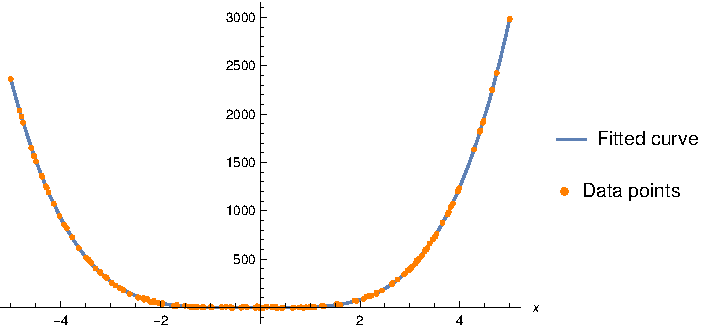
\includegraphics[width=11cm]{legendre_09}
\caption{Base de funciones polinomiales grado 4, 50 puntos, $\delta R=\pm 10$,
curva ajustada: $f(x)=0.44101 + 0.439003 x + 0.537231 (-1 + 3 x^2) + 
 0.50968 (-3 x + 5 x^3) + 0.124784 (3 - 30 x^2 + 35 x^4)$.}
\label{fig:poly_50pts}
\end{figure}


\end{document}